\section{KORD Linear Regression with 2-Hour Deltas: Temperature Prediction Analysis}
This analysis implements multivariate time series regression models to predict temperature at Chicago O'Hare International Airport (KORD) across multiple time horizons, incorporating 2-hour change features.\
\begin{itemize}
  \item Base Model: Multivariate Linear Regression
  \item Feature Engineering: Time-lagged features and 2-hour change features
  \item Prediction Horizons: Multiple time windows (1h, 24h, 5d, 5d avg, 30d avg)
  \item Train/Test Split: 80/20
  \item Random State: 42 (for reproducibility)
  \item Validation: Standard train-test split
\end{itemize}

\subsection{1 Hour Ahead Temperature Prediction}
\subsection{Model Performance}
\begin{tabular}{llr}
\toprule
 & Metric & Value \\
\midrule
0 & Root Mean Squared Error (RMSE) & 1.36 \\
1 & Mean Absolute Error (MAE) & 0.91 \\
2 & R^2 Score & 0.98 \\
\bottomrule
\end{tabular}

\subsection{1 Hour Ahead Predictions}
\begin{figure}[htbp]
\centering
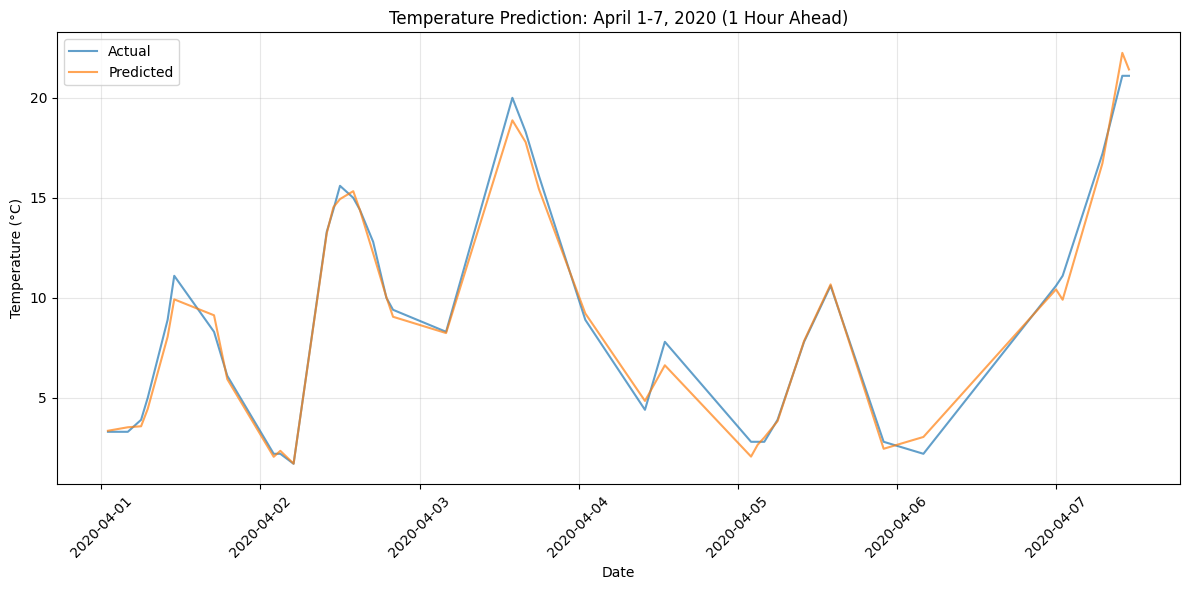
\includegraphics[width=0.7\textwidth]{1-0-linear_temp_shift_results.png}
\caption{1 Hour Ahead Predictions}
\label{fig:1_hour_ahead_pred}
\end{figure}

\subsection{1 Hour Ahead Feature Importance}
\begin{figure}[htbp]
\centering
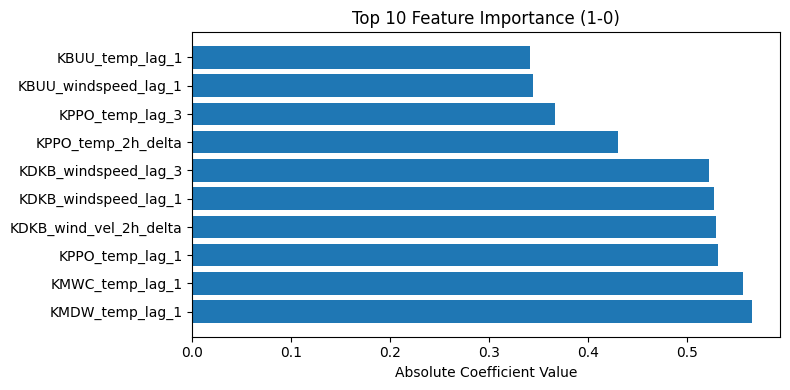
\includegraphics[width=0.7\textwidth]{1-0-linear_temp_shift_feature_importance.png}
\caption{1 Hour Ahead Feature Importance}
\label{fig:1_hour_ahead_featimp}
\end{figure}



\subsection{24 Hours Ahead Temperature Prediction}
\subsection{Model Performance}
\begin{tabular}{llr}
\toprule
 & Metric & Value \\
\midrule
0 & Root Mean Squared Error (RMSE) & 4.72 \\
1 & Mean Absolute Error (MAE) & 3.57 \\
2 & R^2 Score & 0.82 \\
\bottomrule
\end{tabular}

\subsection{24 Hours Ahead Predictions}
\begin{figure}[htbp]
\centering
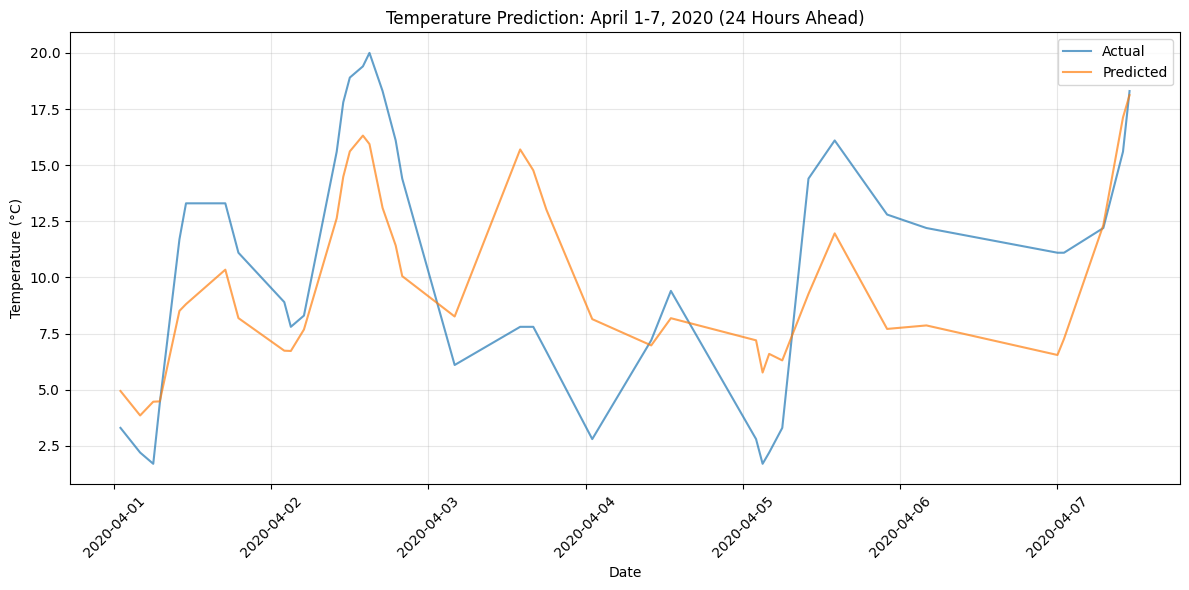
\includegraphics[width=0.7\textwidth]{1-1-linear_temp_shift_results.png}
\caption{24 Hours Ahead Predictions}
\label{fig:24_hours_ahead_pred}
\end{figure}

\subsection{24 Hours Ahead Feature Importance}
\begin{figure}[htbp]
\centering
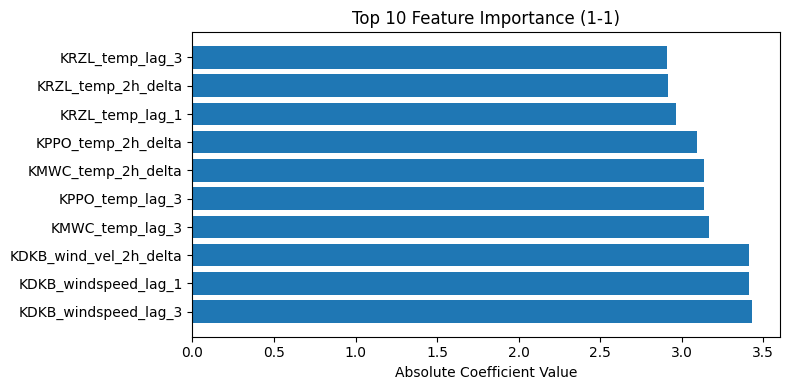
\includegraphics[width=0.7\textwidth]{1-1-linear_temp_shift_feature_importance.png}
\caption{24 Hours Ahead Feature Importance}
\label{fig:24_hours_ahead_featimp}
\end{figure}



\subsection{120 Hours (5 Days) Ahead Temperature Prediction}
\subsection{Model Performance}
\begin{tabular}{llr}
\toprule
 & Metric & Value \\
\midrule
0 & Root Mean Squared Error (RMSE) & 6.31 \\
1 & Mean Absolute Error (MAE) & 4.88 \\
2 & R^2 Score & 0.67 \\
\bottomrule
\end{tabular}

\subsection{120 Hours (5 Days) Ahead Predictions}
\begin{figure}[htbp]
\centering
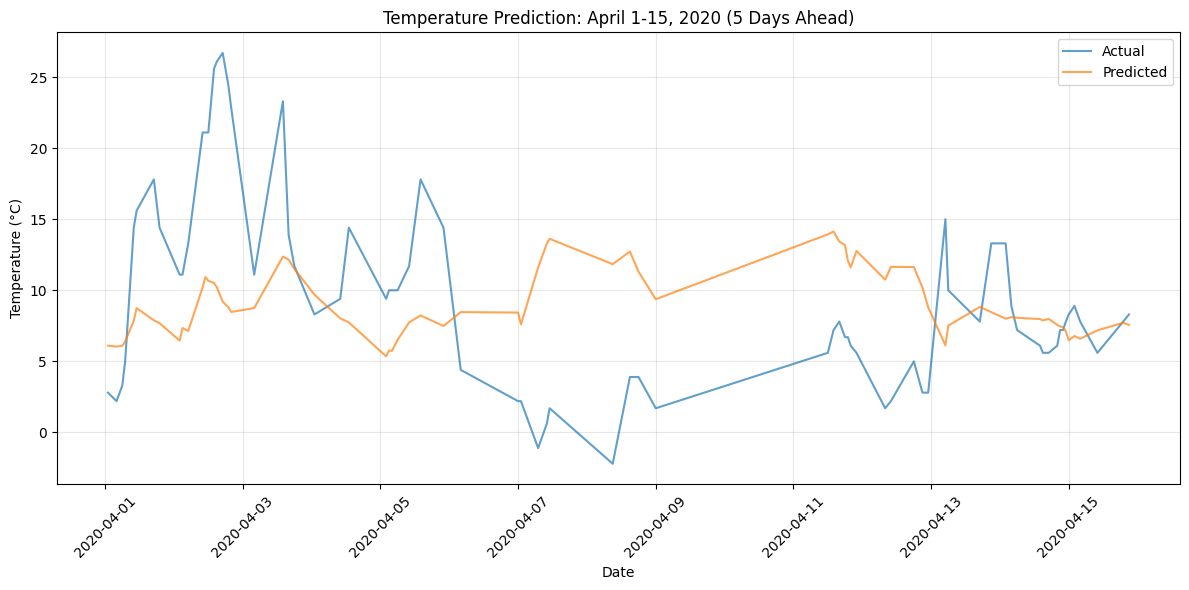
\includegraphics[width=0.7\textwidth]{1-2-linear_temp_shift_results.png}
\caption{120 Hours (5 Days) Ahead Predictions}
\label{fig:120_hours_(5_days)_ahead_pred}
\end{figure}

\subsection{120 Hours (5 Days) Ahead Feature Importance}
\begin{figure}[htbp]
\centering
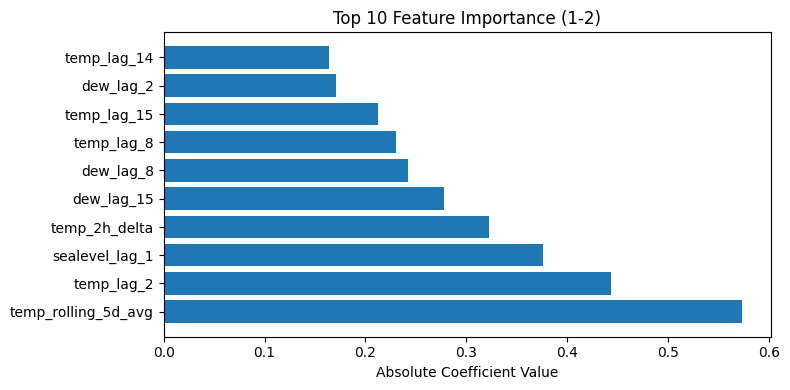
\includegraphics[width=0.7\textwidth]{1-2-linear_temp_shift_feature_importance.png}
\caption{120 Hours (5 Days) Ahead Feature Importance}
\label{fig:120_hours_(5_days)_ahead_featimp}
\end{figure}



\subsection{5-Day Average Ahead Temperature Prediction}
\subsection{Model Performance}
\begin{tabular}{llr}
\toprule
 & Metric & Value \\
\midrule
0 & Root Mean Squared Error (RMSE) & 3.64 \\
1 & Mean Absolute Error (MAE) & 2.81 \\
2 & R^2 Score & 0.87 \\
\bottomrule
\end{tabular}

\subsection{5-Day Average Ahead Predictions}
\begin{figure}[htbp]
\centering
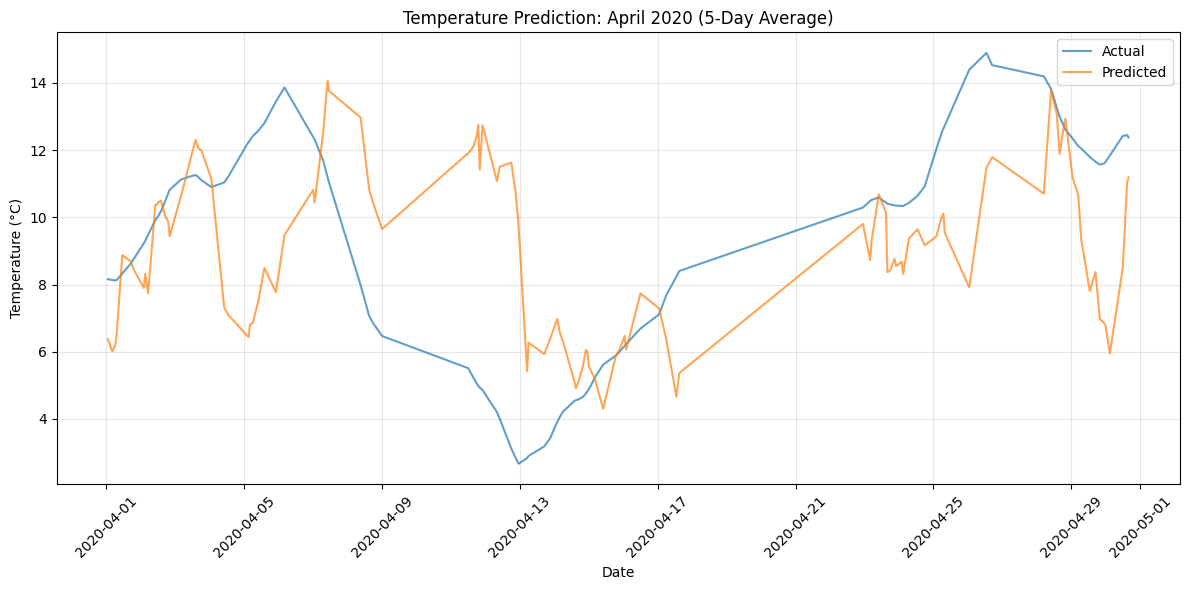
\includegraphics[width=0.7\textwidth]{1-3-linear_temp_shift_results.png}
\caption{5-Day Average Ahead Predictions}
\label{fig:5-day_average_ahead_pred}
\end{figure}

\subsection{5-Day Average Ahead Feature Importance}
\begin{figure}[htbp]
\centering
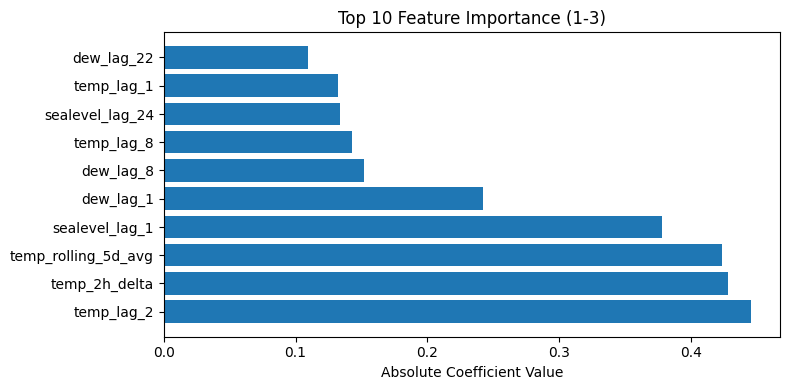
\includegraphics[width=0.7\textwidth]{1-3-linear_temp_shift_feature_importance.png}
\caption{5-Day Average Ahead Feature Importance}
\label{fig:5-day_average_ahead_featimp}
\end{figure}



\subsection{30-Day Average Ahead Temperature Prediction}
\subsection{Model Performance}
\begin{tabular}{llr}
\toprule
 & Metric & Value \\
\midrule
0 & Root Mean Squared Error (RMSE) & 4.53 \\
1 & Mean Absolute Error (MAE) & 3.65 \\
2 & R^2 Score & 0.77 \\
\bottomrule
\end{tabular}

\subsection{30-Day Average Ahead Predictions}
\begin{figure}[htbp]
\centering
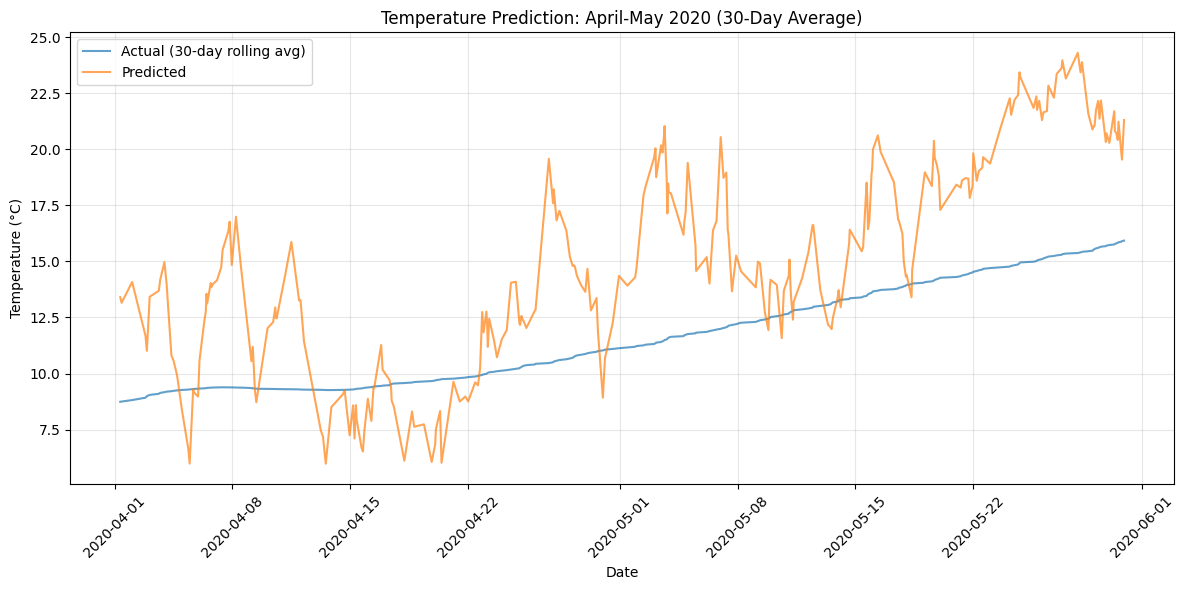
\includegraphics[width=0.7\textwidth]{1-4-linear_temp_shift_results.png}
\caption{30-Day Average Ahead Predictions}
\label{fig:30-day_average_ahead_pred}
\end{figure}

\subsection{30-Day Average Ahead Feature Importance}
\begin{figure}[htbp]
\centering
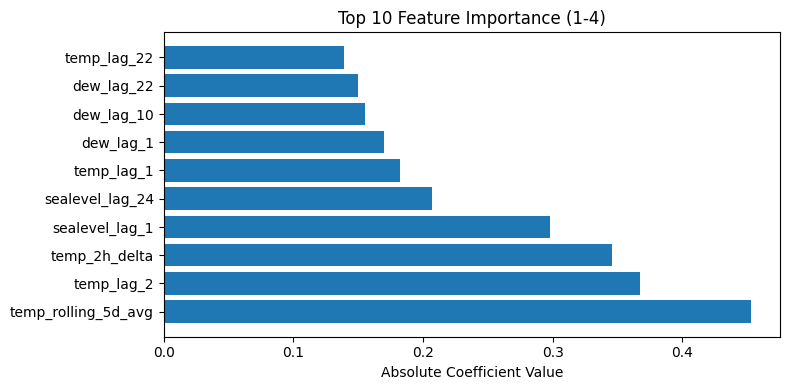
\includegraphics[width=0.7\textwidth]{1-4-linear_temp_shift_feature_importance.png}
\caption{30-Day Average Ahead Feature Importance}
\label{fig:30-day_average_ahead_featimp}
\end{figure}


\section{Model Interpretation}

These multivariate regression models capture the complex relationships between various weather parameters and temperature across different time horizons. The models:\
\begin{itemize}
  \item Consider the impact of all available weather parameters
  \item Account for changes in temperature, wind direction, and wind velocity over 2-hour periods
  \item Provide insights into which factors most influence temperature at different time scales
\end{itemize}
Future improvements could include:\
\begin{itemize}
  \item Feature selection to reduce dimensionality
  \item Non-linear models to capture complex relationships
  \item Time series specific models (ARIMA, LSTM)
\end{itemize}

